\documentclass[border=5mm]{standalone}
\usepackage[T1]{fontenc}
\usepackage[scaled]{helvet}
\renewcommand\familydefault{\sfdefault}
\usepackage{tikz}
\usepackage{xcolor}
\usetikzlibrary{positioning, fit, backgrounds}

\definecolor{ink}{HTML}{20272E}
\definecolor{teal}{HTML}{0E7C86}
\definecolor{coral}{HTML}{C0392B}
\definecolor{sand}{HTML}{F3F0E7}
\definecolor{muted}{HTML}{6B7680}

\newcommand{\tile}[4]{% x-center, fill, BIG, label
  \begin{scope}
  \node[rounded corners=4pt, fill=#2, minimum width=5.3cm, minimum height=3.5cm,
        anchor=north, inner sep=9pt, text width=4.6cm, align=left, text=white] (t) at (#1,9.4) {};
  \node[anchor=north west, text=white, font=\fontsize{30}{30}\selectfont\bfseries]
        at ([xshift=9pt,yshift=-8pt]t.north west) {#3};
  \node[anchor=south west, text=white, font=\fontsize{10.5}{12.5}\selectfont, text width=4.5cm, align=left]
        at ([xshift=9pt,yshift=9pt]t.south west) {#4};
  \end{scope}}

\begin{document}
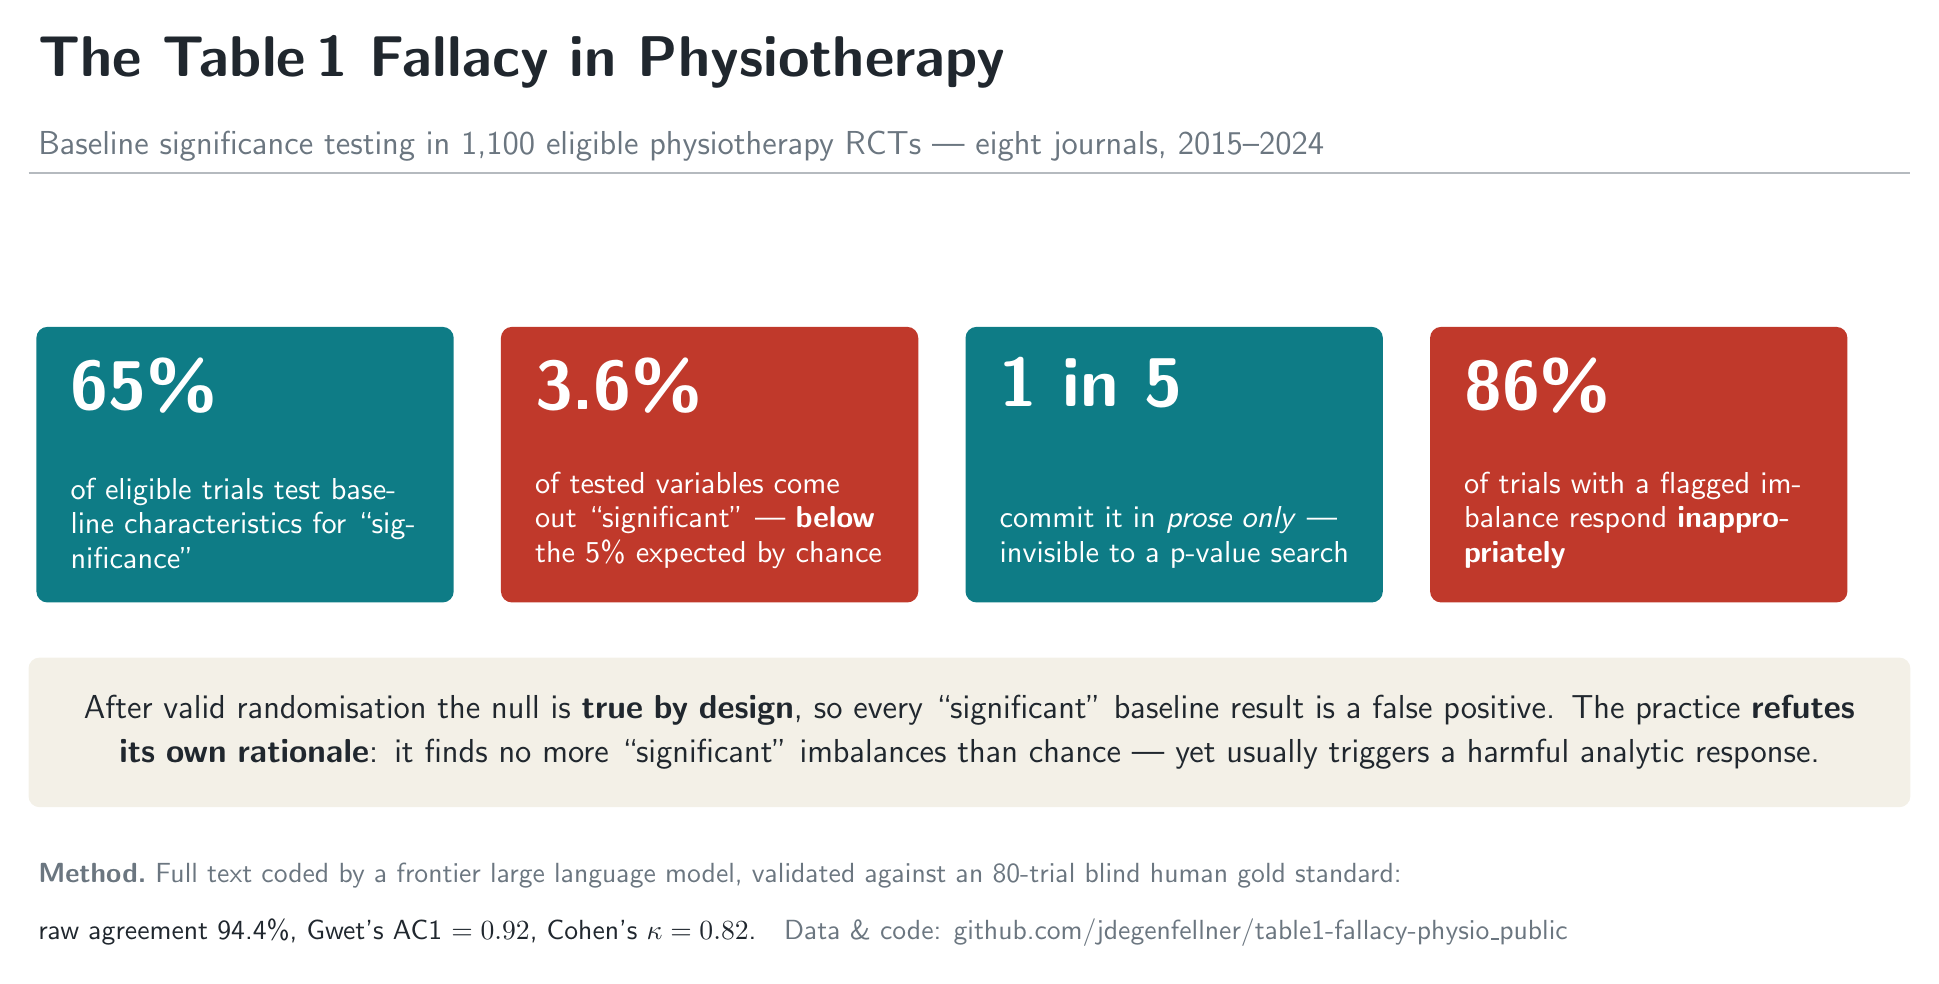
\begin{tikzpicture}[font=\sffamily]
% ---- header ----
\node[anchor=north west, text=ink, font=\fontsize{22}{24}\selectfont\bfseries] (h)
  at (0,13.2) {The Table\,1 Fallacy in Physiotherapy};
\node[anchor=north west, text=muted, font=\fontsize{12}{14}\selectfont]
  at (0,12.0) {Baseline significance testing in 1{,}100 eligible physiotherapy RCTs --- eight journals, 2015--2024};
\draw[muted!50, line width=0.6pt] (0,11.35) -- (23.9,11.35);

% ---- four stat tiles ----
\tile{2.75}{teal}{65\%}{of eligible trials test baseline characteristics for ``significance''}
\tile{8.65}{coral}{3.6\%}{of tested variables come out ``significant'' --- \textbf{below} the 5\% expected by chance}
\tile{14.55}{teal}{1 in 5}{commit it in \emph{prose only} --- invisible to a p-value search}
\tile{20.45}{coral}{86\%}{of trials with a flagged imbalance respond \textbf{inappropriately}}

% ---- punch line band ----
\node[rounded corners=4pt, fill=sand, minimum width=23.9cm, minimum height=1.9cm,
      anchor=north, inner sep=10pt, text width=22.8cm, align=center, text=ink,
      font=\fontsize{13}{16}\selectfont] at (11.95,5.2)
  {After valid randomisation the null is \textbf{true by design}, so every ``significant'' baseline
   result is a false positive. The practice \textbf{refutes its own rationale}: it finds no more
   ``significant'' imbalances than chance --- yet usually triggers a harmful analytic response.};

% ---- method footer ----
\node[anchor=north west, text=muted, font=\fontsize{10}{12}\selectfont] at (0,2.7)
  {\textbf{Method.}~Full text coded by a frontier large language model, validated against an
   80-trial blind human gold standard:};
\node[anchor=north west, text=ink, font=\fontsize{10}{12}\selectfont] at (0,2.0)
  {raw agreement 94.4\%, Gwet's AC1 $=0.92$, Cohen's $\kappa=0.82$.\quad
   \textcolor{muted}{Data \& code: github.com/jdegenfellner/table1-fallacy-physio\_public}};
\end{tikzpicture}
\end{document}
